% Chapter Template

\chapter{Sistemas de Detección de Intrusiones} % Main chapter title

\label{Chapter2} % Change X to a consecutive number; for referencing this chapter elsewhere, use \ref{ChapterX}

%----------------------------------------------------------------------------------------
%	SECTION 1
%----------------------------------------------------------------------------------------

\section{Qué son los IDS}
Tal y como se ha visto en el capítulo anterior, la llegada de Internet y su extensión en todo tipo de ámbitos ha supuesto, además de un gran avance, la introducción de ciertos riesgos y vulnerabilidades, antes inexistentes. A día de hoy resulta inconcebible que una empresa de cierto tamaño no cuente con su propia red o utilice Internet para llevar a cabo gran parte de su actividad. Las facilidades que esta apertura al exterior puede proporcionar se contraponen con los ataques que estas organizaciones son susceptibles de sufrir. Pese a que existen soluciones que tratan de garantizar la seguridad y que únicamente los usuarios autorizados accedan a los recursos, dichas soluciones no resultan infalibles y dependen, además, de tareas de mantenimiento que están sujetas a fallos u olvidos. Es ahí donde entran en juego los IDS o  sistemas de detección de intrusiones\cite{Kemmerer}.
Una vez que el atacante ha traspasado las medidas de prevención resulta esencial detectarlo por las siguientes razones:
\begin{itemize}
	\item Cuanto antes se localice la intrusión, antes se pueden tomar medidas al respecto y, por lo tanto, menor será el daño causado por el ataque.
	\item De la misma manera que un sistema de alarmas instalado en una casa puede disuadir a ladrones a la hora de perpetrar un robo, un IDS también puede frenar posibles ataques.
	\item La detección de ataques proporciona una gran cantidad de información sobre las estrategias empleadas por los atacantes, y contribuyen a solventar vulnerabilidades del sistema de prevención.
\end{itemize}
En un paso previo a la descripción de los sistemas de detección de intrusiones, a continuación se explican los riesgos y los distintos ataques que puede sufrir un sistema. Dejando al margen los virus, que junto con las intrusiones representan los ataques más comunes, podrían distinguirse distintos tipos de intrusos\cite{Stallings2016}:
\begin{itemize}
	\item \textbf{Impostor}: en este caso el intruso entra en el sistema bajo la identidad de un usuario legitimo y hace uso de los recursos de dicha cuenta.
	\item \textbf{Usuario negligente}: un usuario legitimo del sistema utiliza de manera errónea o abusiva los recursos a los que tiene acceso, ya sean datos o programas.
	\item \textbf{Usuario clandestino}. Se trata de un atacante que intenta apropiarse de los privilegios del administrador o superusuario. Bajo la identidad del administrador el atacante puede, además, eludir controles de acceso o el registro de sus actividades.
\end{itemize}
%-----------------------------------
%	SUBSECTION 1
%-----------------------------------
\subsection{Tipos de IDS}
Existen dos criterios para clasificar los IDS: según dónde se coloquen o según la técnica que empleen. Atendiendo al punto de la red en que se encuentre, hay:
\begin{itemize}
	\item \textbf{IDSs basados en \textit{host} o máquina}: se localizan a nivel de una única máquina, corriendo como aplicaciones, y analizan ficheros de log para detectar intrusiones.
	\item \textbf{IDSs basados en red}: este tipo de IDS se encuentra en puntos concretos de la red, ya sea a la entrada o en el área desmilitarizada \textit{DMZ}. En este caso se analiza todo el tráfico de la red y no solamente el que llega a cierta máquina.
	\item \textbf{IDSs híbridos}: en este caso se combinan las dos modalidades previamente mencionadas.
\end{itemize}
Por otro, en función de la técnica que se utilice para detectar la intrusión, se encuentran los siguientes IDSs:
\begin{itemize}
	\item \textbf{Detección por uso inadecuado o basada en conocimiento}: se buscan trazas de ataques, patrones en el tráfico de red o registros en logs que puedan denotar un comportamiento sospechoso. Este tipo de sistema reconocería como sospechoso un número elevado de intentos fallidos de acceso.
	\item \textbf{Detección por firma}: En este caso, se monitorizan los paquetes de la red, comparándolos con patrones predeterminados y reconocidos, que se conocen como firmas. Ante la detección de un nuevo ataque, expertos extraen características que se traducen en firmas y permitan su detección en futuras ocasiones. Este tipo de sistemas presenta como inconveniente el lapso de tiempo que transcurre entre que se detecta un ataque y la firma está disponible.
	\item \textbf{Detección por anomalía}: la instrusión es detectada cuando se identifica un comportamiento anómalo para determinado perfil o se superan los umbrales fijados según análisis estadísticos. Algunos ejemplos de los ataques que se pueden detectar serían suplantación de la identidad o un ataque de denegación de servicio. 
\end{itemize}
\cite{Vuppala}
%\begin{figure}[t]
%\centering
%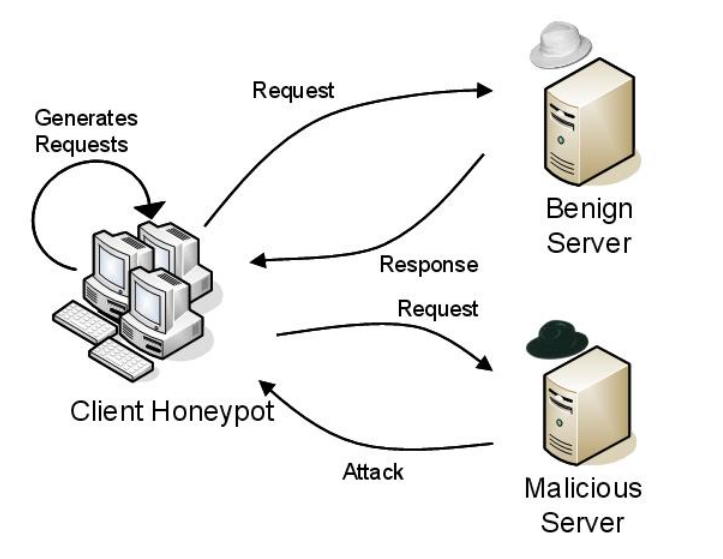
\includegraphics[width=0.8\textwidth]{images/clienthoneypot.png}
%\caption{Funcionamiento de un cliente \textit{honeypot}}
%\label{fig:clienthoneypot}
%\end{figure}
